
\chapter{Running PyLith}

Figure \vref{fig:pylith:workflow} shows the workflow for running PyLith.
There are essentially three main inputs needed to run a problem with
PyLith:
\begin{enumerate}
\item Mesh information. This includes the topology of the
  finite-element mesh (coordinates of vertices and how the vertices
  are connected into cells), a material identifier for each cell, and
  sets of vertices associated with boundary conditions, faults, and
  output (for subsets of the mesh). This information can be provided
  using the PyLith mesh ASCII format (see Chapter \vref{sec:examples}
  for examples and Section \vref{sec:MeshIOAscii} for the format
  specification) or by importing the information from the LaGriT or
  CUBIT meshing packages (see Chapter \vref{src:examples} for
  examples).
\item A set of parameters describing the problem. These parameters
  describe the type of problem to be run, solver information,
  time-stepping information, boundary conditions, materials, etc. This
  information can be provided from the command-line or by using a
  \filename{.cfg.}
\item Databases specifying the material property values and boundary
  condition values to be used. Arbitrarily complex spatial variations
  in boundary and fault conditions and material properties may be
  given in the spatial database (see Chapter \vref{sec:examples} for
  examples and Appendix \vref{sec:spatialdata:SimpleIOAscii} for the
  format specification).
\end{enumerate}
PyLith writes solution information, such as solution fields and state
variables, to either VTK files or HDF5/Xdmf files. ParaView and Visit
can read both types of files. Post-processing of output is generally
performed using HDF5 files accessed via a Python script and the h5py
package or a Matlab script.

\begin{figure}[htbp]
  \includegraphics[width=5in]{runpylith/figs/runpylith} 
  \caption{PyLith requires a finite-element mesh (three different
    mechanisms for generating a mesh are currently supported),
    simulation parameters, and spatial databases (defining the spatial
    variation of various parameters).  PyLith writes the solution
    output to either VTK or HDF5/Xdmf files, which can be visualized
    with ParaView or Visit. Post-processing is generally done using
    the HDF5 files with Python or Matlab scripts.}
\label{fig:pylith:workflow} 
\end{figure}


\section{Defining the Simulation}

The parameters for PyLith are specified as a hierarchy or tree of
modules. The application assembles the hierarchy of modules from user
input and then calls the \object{main} function in the top-level
module in the same manner as a C or C++ program. The behavior of the
application is determined by the modules included in the hierarchy as
specified by the user. The Pyre framework provides the interface for
defining this hierarchy. Pyre properties correspond to simple settings
in the form of strings, integers, and real numbers. Pyre facilities
correspond to software modules. Facilities may have their own
facilities (branches in the tree) and any number of properties. See
Figure \vref{fig:Pyre:Architecture} for the general concept of Pyre
facilities and properties. The top-level object is the PyLith
application with three facilities: \facility{mesher}, \facility{problem},
and \facility{petsc}. The \facility{mesher} specifies how to import the
mesh, the \facility{problem} specifies the physical properties, boundary
conditions, etc., and \facility{petsc} is used to specify PETSc
settings. Appendix \vref{sec:components} contains a list of the
components provided by PyLith and spatialdata.


\subsection{Setting PyLith Parameters}
\label{sec:setting:parameters}

There are several methods for setting input parameters for the
\filename{pylith} executable: via the command line or by using a text
file in \filename{.cfg} or \filename{.pml} format. Both facilities and
properties have default values provided, so you only need to set
values when you want to deviate from the default behavior.


\subsubsection{Units}

All dimensional parameters require units. The units are specified
using Python and FORTRAN syntax, so square meters is m**2. Whitespace
is not allowed in the string, for units and dimensioned quantities
are multiplied by the units string; for example, two meters per second
is 2.0*m/s. Available units are shown in Table \vref{tab:pyre:units}

\begin{table}[htbp]
\caption{Pyre supported units. Aliases are in parentheses.}
\label{tab:pyre:units}
\begin{tabular}{lp{5in}}
\textbf{Scale} & \textbf{Available Units} \\
\hline 
length & meter (m), micrometer (um, micron), millimeter (mm), centimeter (cm),
kilometer (km), inch, foot, yard, mile \\
time & second (s), nanosecond (ns), microsecond (us), millisecond (ms), minute,
hour, day, year \\
mass & kilogram (kg), gram (g), centigram (cg), milligram (mg), ounce, pound,
ton \\
pressure & pascal (Pa), kPa, MPa, GPa, bar, millibar, atmosphere (atm) \\
\hline 
\end{tabular}
\end{table}


\subsubsection{Using the Command Line}

The \commandline{-{}-help} command line argument displays links to useful
resources for learning PyLith.

Pyre uses the following syntax to change properties from the command
line. To change the value of a property of a component, use
\commandline{-{}-COMPONENT.PROPERTY=VALUE}. Each component is attached
to a facility, so the option above can also be written as
\commandline{-{}-FACILITY.PROPERTY=VALUE}.  Each facility has a
default component attached to it. A different component can be
attached to a facility by \commandline{-{}-FACILITY=NEW\_COMPONENT}.

PyLith's command-line arguments can control Pyre and PyLith properties
and facilities, MPI settings, and PETSc settings. All PyLith-related
properties are associated with the \facility{pylithapp} component. You
can get a list of all of these top-level properties along with a
description of what they do by running PyLith with the
\commandline{-{}-help-properties} command-line argument. To get
information on user-configurable facilities and components, you can
run PyLith with the \commandline{-{}-help-components} command-line
argument. To find out about the properties associated with a given
component, you can run PyLith with the
\commandline{-{}-COMPONENT.help-properties} flag:
\begin{shell}
$$ pylith -{}-problem.help-properties
# Show problem components.
$$ pylith -{}-~problem.help-components
# Show bc components (bc is a component of problem).
$$ pylith -{}-problem.bc.help-components
# Show bc properties.
$$ pylith -{}-problem.bc.help-properties
\end{shell}


\subsubsection{Using a {\ttfamily .cfg} File}

Entering all those parameters via the command line involves the risk
of typographical errors. You
will generally find it easier to collect parameters into a
\filename{.cfg} file. The file is composed of one or more sections
which are formatted as follows:
\begin{cfg}
<h>[pylithapp.COMPONENT1.COMPONENT2]</h>
# This is a comment.

<f>FACILITY3</f> = COMPONENT3
<p>PROPERTY1</p> = VALUE1
<p>PROPERTY2</p> = VALUE2 ; this is another comment
\end{cfg}

\tip{We strongly recommend that you use \filename{.cfg} files for your
  work.  The files are syntax-highlighted in the vim editor.}


\subsubsection{Using a {\ttfamily.pml} File}

A \filename{.pml} file is an XML file that specifies parameter values
in a highly structured format. It is composed of nested sections which
are formatted as follows:
\begin{lstlisting}[basicstyle=\ttfamily,frame=tb]{language=xml}
<component~name="COMPONENT1">
    <component~name="COMPONENT2">
        <property~name="PROPERTY1">VALUE1</property>
        <property~name="PROPERTY2">VALUE2</property>
    </component>
</component>
\end{lstlisting}
XML files are intended to be read and written by machines, not edited
manually by humans. The \filename{.pml} file format is intended for
applications in which PyLith input files are generated by another
program, e.g., a GUI, web application, or a high-level structured
editor. This file format will not be discussed further here, but if
you are interested in using \filename{.pml} files, note that \filename{.pml}
files and \filename{.cfg} files can be used interchangeably; in the
following discussion, a file with a \filename{.pml} extension can be
substituted anywhere a \filename{.cfg} file can be used.


\subsubsection{Specification and Placement of Configuration Files}

Configuration files may be specified on the command line:
\begin{shell}
$$ pylith example.cfg
\end{shell}
In addition, the Pyre framework searches for configuration files named
\filename{pylithapp.cfg} in several predefined locations. You may put
settings in any or all of these locations, depending on the scope
you want the settings to have:
\begin{enumerate}
\item \filename{\$PREFIX/etc/pylithapp.cfg}, for system-wide settings;
\item \filename{\$HOME/.pyre/pylithapp/pylithapp.cfg}, for user
  settings and preferences;
\item the current directory (\filename{./pylithapp.cfg}), for local
  overrides.
\end{enumerate}

\important{The Pyre framework will search these directories for
  \filename{.cfg} files matching the names of components (for example,
  \filename{timedependent.cfg}, \filename{faultcohesivekin.cfg},
  \filename{greensfns.cfg}, \filename{pointforce.cfg}, etc) and will
  attempt to assign all parameters in those files to the respective
  component.}

\important{Parameters given directly on the command line will override
  any input contained in a configuration file. Configuration files
  given on the command line override all others. The
  \filename{pylithapp.cfg} files placed in (3) will override those in
  (2), (2) overrides (1), and (1) overrides only the built-in
  defaults.}

All of the example problems are set up using configuration files and specific problems are defined by including
the appropriate configuration file on the command-line. Referring
to the directory \filename{examples/twocells/twohex8}, we have the
following.
\begin{shell}
$$ ls -1 *.cfg
axialdisp.cfg
dislocation.cfg
pylithapp.cfg
sheardisp.cfg
\end{shell}
The settings in \filename{pylithapp.cfg} will be read automatically, and additional
settings are included by specifying one of the other files on the
command-line:
\begin{shell}
$$ pylith axialdisp.cfg
\end{shell}
If you want to see what settings are being used, you can either examine
the \filename{.cfg} files, or use the help flags as described above:
\begin{shell}
# Show components for the 'problem' facility.
$$ pylith axialdisp.cfg --problem.help-components
# Show properties for the 'problem' facility.
$$ pylith axialdisp.cfg --problem.help-properties
# Show components for the 'bc' facility.
$$ pylith axialdisp.cfg --problem.bc.help-components
# Show properties for the 'bc' facility.
$$ pylith axialdisp.cfg --problem.bc.help-properties
\end{shell}
This is generally a more useful way of determining problem settings,
since it includes default values as well as those that have been specified
in the \filename{.cfg} file.


\subsubsection{List of PyLith Parameters ({\ttfamily pylithinfo})}

The Python application \filename{pylithinfo} writes all of the current
parameters to a text file. The default name of the text file is \filename{pylith\_parameters.txt}.
The usage synopsis is
\begin{shell}
$$ pylithinfo --verbose [--fileout=pylith_parameters.txt] PYLITH_ARGS
\end{shell}
where \commandline{-{}-verbose} turns on printing the descriptions of
the properties and components as well as the location where the
current value was set, and
\commandline{-{}-fileout=pylith\_parameters.txt} sets the name of the
output file. The lines in the text file are indented to show the
hierarchy of the properties and component.


\subsection{Mesh Information (\facility{mesher})}

Geometrical and topological information for the finite element mesh
may be provided by exporting an Exodus II format file from
CUBIT/Trelis, by exporting a GMV file and an accompanying Pset file
from LaGriT, or by specifying the information in PyLith mesh ASCII
format. See Chapter \vref{cha:examples} for examples.

PyLith supports linear cells in 2D (Figure \vref{fig:2D:cells}), and
3D (Figure \vref{fig:3D:cells}).  The vertex ordering must follow the
convention shown in Figures \vref{fig:2D:cells}-\vref{fig:3D:cells}.
PyLith no longer supports use of quadratic cells using the PyLith
ASCII mesh format. In the next release, we plan to support higher
order discretizations via PETSc finite-element features from meshes
with linear cells as input.

The mesh information defines the vertex coordinates and specifies
the vertices composing each cell in the mesh. The mesh information
must also define at least one set of vertices for which displacement
(Dirichlet) boundary conditions will be provided. In most realistic
problems, there will be several vertex groups, each with a unique
identifying label. For example, one group might define a surface of
the mesh where displacement (Dirichlet) boundary conditions will be
applied, another might define a surface where traction (Neumann) boundary
conditions will be applied, while a third might specify a surface
that defines a fault. Similarly, the mesh information contains cell
labels that define the material type for each cell in the mesh. For
a mesh with a single material type, there will only be a single label
for every cell in the mesh. See Chapters \vref{cha:material:models}
and \vref{cha:boundary:interface:conditions} for more detailed discussions
of setting the materials and boundary conditions.

\begin{figure}[htbp]
  \includegraphics{runpylith/figs/tri3}\hspace*{0.5in}%
  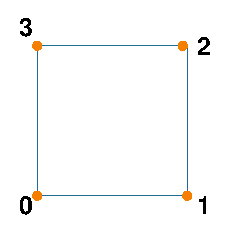
\includegraphics{runpylith/figs/quad4}
  \caption{Linear cells available for 2D problems are the triangle
    (left) and the quadrilateral (right).}
  \label{fig:2D:cells}
\end{figure}

\begin{figure}[htbp]
  \includegraphics{runpylith/figs/tet4}\hspace*{0.5in}%
  \includegraphics{runpylith/figs/hex8}
  \caption{Linear cells available for 3D problems are the tetrahedron (left)
    and the hexahedron (right).}
  \label{fig:3D:cells}
\end{figure}

\subsubsection{\object{Mesh Importer}}

The default mesher component is \object{MeshImporter}, which provides
the capabilities of reading the mesh from files. The \object{MeshImporter} has
several properties and facilities:
\begin{inventory}
  \propertyitem{reorder\_mesh}{Reorder the vertices and cells using the
    reverse Cuthill-McKee algorithm (default is False)}
  \facilityitem{reader}{Reader for a given type of mesh (default is
    \object{MeshIOAscii}).}
  \facilityitem{distributor}{Handles
    distribution of the mesh among processors.}
  \facilityitem{refiner}{Perform global uniform mesh refinement after
    distribution among processors (default is no refinement).}
\end{inventory}
Reordering the mesh so that vertices and cells connected topologically
also reside close together in memory improves overall performance
and can improve solver performance as well.

\warning{The coordinate system associated with the mesh must be a
  Cartesian coordinate system, such as a generic Cartesian coordinate
  system or a geographic projection.}

\subsubsection{\object{MeshIOAscii}}

The \object{MeshIOAscii} object is intended for reading small, simple
ASCII files containing a mesh constructed by hand. We use this file
format extensively in the examples. Appendix \vref{sec:MeshIOAscii}
describes the format of the files. The properties and facilities of
the \object{MeshIOAscii} object include:
\begin{inventory}
\propertyitem{filename}{Name of the mesh file.}
\facilityitem{coordsys}{Coordinate system associated with the mesh.}
\end{inventory}

\subsubsection{\object{MeshIOCubit}}
\label{sec:MeshIOCubit}

The \object{MeshIOCubit} object reads the NetCDF Exodus II files output from
CUBIT/Trelis. Beginning with CUBIT 11.0, the names of the nodesets are included
in the Exodus II files and PyLith can use these nodeset names or revert
to using the nodeset ids. The properties and facilities associated
with the \object{MeshIOCubit} object are:
\begin{inventory}
\propertyitem{filename}{Name of the Exodus II file.}
\propertyitem{use\_nodeset\_names}{Identify nodesets by name rather than id
(default is True).}
\facilityitem{coordsys}{Coordinate system associated with the mesh.}
\end{inventory}

\subsubsection{\object{MeshIOLagrit}}
\label{sec:MeshIOLagrit}

The \object{MeshIOLagrit} object is used to read ASCII and binary GMV and PSET
files output from LaGriT. PyLith will automatically detect whether
the files are ASCII or binary. We attempt to provide support for experimental
64-bit versions of LaGriT via flags indicating whether the FORTRAN
code is using 32-bit or 64-bit integers. The \object{MeshIOLagrit} properties
and facilities are:
\begin{inventory}
  \propertyitem{filename\_gmv}{Name of GMV file.}
  \propertyitem{filename\_pset}{Name of the PSET file.}
  \propertyitem{flip\_endian}{Flip the endian of values when reading
    binary files (default is False).}
  \propertyitem{io\_int32}{Flag
    indicating that PSET files use 32-bit integers (default is True).}
  \propertyitem{record\_header\_32bt}{Flag indicating FORTRAN record header is
    32-bit (default is True).}
\facilityitem{coordsys}{Coordinate system associated with mesh.}
\end{inventory}

\warning{The PyLith developers have not used LaGriT since around 2008
  and the most recent release appears to have been in 2010.}

\subsubsection{\object{Distributor}}

The distributor uses a partitioner to compute which cells should be
placed on each processor, computes the overlap among the processors,
and then distributes the mesh among the processors. The type of
partitioner is set via PETSc settings. The properties and facilities
of the \object{Distributor} include:
\begin{inventory}
\propertyitem{partitioner}{Name of mesh partitioner ['chaco','parmetis'].}
\propertyitem{write\_partition}{Flag indicating that the partition information
should be written to a file (default is False).}
\facilityitem{data\_writer}{Writer for partition information (default
  is \object{DataWriterVTK} for VTK output).}
\end{inventory}
An example of setting the partitioner in a \filename{pylithapp.cfg}
  file is:
\begin{cfg}
<h>[pylithapp.mesh_generator.distributor]</h>
<p>partitioner</p> = chaco ; Options are 'chaco' (default) and 'parmetis'.
\end{cfg}
METIS/ParMETIS are not included in the PyLith binaries due to licensing
issues. 


\subsubsection{\object{Refiner}}

The refiner is used to decrease node spacing by a power of two by
recursively subdividing each cell by a factor of two. In a 2D triangular
mesh a node is inserted at the midpoint of each edge, splitting each
cell into four cells (see Figure \vref{fig:uniform:refinement:2x}).
In a 2D quadrilateral mesh a node is inserted at the midpoint of each
edge and at the centroid of the cell, splitting each cell into four
cells. In a 3D tetrahedral mesh a node is inserted at the midpoint
of each edge, splitting each cell into eight cells. In a 3D hexahedral
mesh a node is inserted at the midpoint of each edge, the centroid
of each face, and at the centroid of the cell, splitting each cell
into eight cells.

\begin{figure}[htbp]
  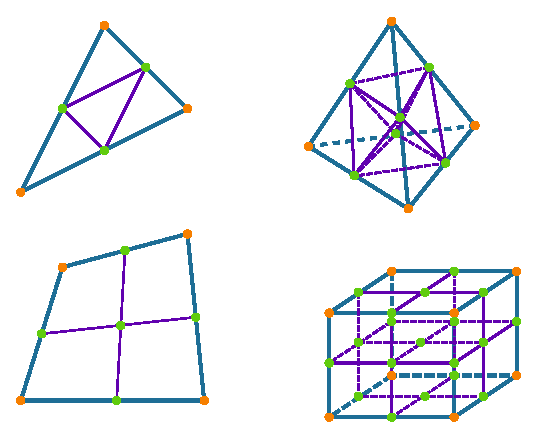
\includegraphics[scale=1.25]{runpylith/figs/refinement2x}
  \caption{Global uniform mesh refinement of 2D and 3D linear
    cells. The blue lines and orange circles identify the edges and
    vertices in the original cells. The purple lines and green circles
    identify the new edges and vertices added to the original cells to
    refine the mesh by a factor of two.}
\label{fig:uniform:refinement:2x}
\end{figure}

Refinement occurs after distribution of the mesh among processors.
This allows one to run much larger simulations by (1) permitting the
mesh generator to construct a mesh with a node spacing largeer than
that needed in the simulation and (2) operations performed in serial
during the simulation setup phase, such as, adjusting the topology
to insert cohesive cells and distribution of the mesh among processors
uses this much smaller coarse mesh. For 2D problems the global mesh
refinement increases the maximum problem size by a factor of $4^{n}$,
and for 3D problems it increases the maximum problem size by a factor
of $8^{n}$, where $n$ is the number of recursive refinement levels.
For a tetrahedral mesh, the element quality decreases with refinement
so $n$ should be limited to 1-2.


\subsection{Problem Specification (\facility{problem})}

The problem component specifies the basic parameters of the simulation,
including the physical properties, the boundary conditions, and interface
conditions (faults). The current release of PyLith contains two types
of problems, \object{TimeDependent} for use in static, quasi-static,
and dynamic simulations and \object{GreensFns} for computing static
Green's functions. The general properties facilities include:
\begin{inventory}
  \propertyitem{dimension}{Spatial dimension of problem space.}
  \facilityitem{normalizer}{Scales used to nondimensionalize the
    problem (default is \object{NondimElasticQuasistatic}).}
  \facilityitem{materials}{Array of materials comprising the domain
    (default is [material]).}
  \facilityitem{bc}{Array of boundary conditions (default is none).}
  \facilityitem{interfaces}{Array of interface conditions, i.e., faults
    (default is none).}
  \facilityitem{gravity\_field}{Gravity field used to construct body
    forces (default is none).}
  \facilityitem{progress\_ monitor}{Show progress of running
    simulation.}
\end{inventory}
An example of setting these parameters in a \filename{.cfg} file for
a problem is:
\begin{cfg}
<h>[pylithapp.timedependent]</h>
<p>dimension</p> = 3
<f>normalizer</f> = spatialdata.units.NondimElasticQuasistatic
<f>materials</f> = [elastic, viscoelastic]
<f>bc</f> = [boundary_east, boundary_bottom, boundary_west]
<f>interfaces</f> = [SanAndreas, SanJacinto]
<f>gravity_field</f> = spatialdata.spatialdb.GravityField
\end{cfg}

\subsubsection{Nondimensionalization (\facility{normalizer})}

PyLith nondimensionalizes all parameters provided by the user so that
the simulation solves the equations using nondimensional quantities.
This permits application of PyLith to problems across a vast range
of spatial and temporal scales. The scales used to nondimensionalize
the problem are length, pressure, density, and time. PyLith provides
two normalizer objects to make it easy to provide reasonable scales
for the nondimensionalization. The \object{NondimElasticQuasistatic}
normalizer (which is the default) has the following properties:
\begin{inventory}
  \propertyitem{length\_scale}{Distance to nondimensionalize length
    (default is 1.0 km).}
  \propertyitem{shear\_modulus}{Shear modulus to nondimensionalize
    pressure (default is 3.0e+10 Pa).}
  \propertyitem{relaxation\_time}{Relaxation time to
    nondimensionalize time (default is 1.0 year).}
\end{inventory}
An example of setting these parameters in a \filename{.cfg} file for
a problem is:
\begin{cfg}
<h>[pylithapp.timedependent.normalizer]</h>
<p>length_scale</p> = 1.0*km
<p>shear_modulus</p> = 3.0e+10*Pa
<p>relaxation_time</p> = 1.0*yr
\end{cfg}
The \object{NondimElasticDynamic} normalizer has the following
properties:
\begin{inventory}
  \propertyitem{shear\_wave\_speed}{Shear wave speed used to
    nondimensionalize length and pressure (default is 3.0 km/s).}
  \propertyitem{mass\_density}{Mass density to nondimensionalize
    density and pressure (default is 3.0e+3 kg/m$^{3}$).}
  \propertyitem{wave\_period}{Period of seismic waves used to
    nondimensionalize time (default is 1.0 s).}
\end{inventory}
An example of setting these parameters in a \filename{.cfg} file for
a problem is:
\begin{cfg}
<h>[pylithapp.timedependent.normalizer]</h>
<p>shear_wave_speed</p> = 3.0*km/s
<p>mass_density</p> = 3.0e+3*kg/m**3
<p>wave_period</p> = 1.0*s
\end{cfg}

\important{The default nondimensionalization is reasonable for many
  problems; however, it may be necessary to change the default values
  in some cases. When doing this, keep in mind that the
  nondimensionalization generally applies to the minimum values
  encountered for a problem.  For example, in a quasistatic problem,
  the \property{length\_scale} should be on the order of the minimum
  cell size. Similarly, the \property{relaxation\_time} should be on
  the order of the minimum relaxation time.}

\subsection{Finite-Element Integration Settings}

PyLith uses numerical quadrature to evaluate the finite-element integrals
for the residual and system Jacobian (see Chapter \vref{cha:Governing-Equations}).
PyLith employs FIAT (finite element automatic tabulator) to compute
the basis functions and their derivatives at the quadrature points
for various quadrature schemes and cell shapes. The parameters for
Lagrange cells (lines, quadrilaterals, hexahedra) are specified using
the FIATLagrange object, whereas the parameters for Simplex cells
(lines, triangles, tetrahedra) are specified using the FIATSimplex
object. Both objects use the same set of parameters and PyLith will
setup the basis functions and quadrature scheme appropriately for
the two families of cells. The quadrature scheme and basis functions
must be set for each material and boundary condition involving finite-element
integrations (Dirichlet boundary conditions are constraints and do
not involve integrations). Furthermore, the integration schemes can
be set independently. The current version of PyLith supports basis
functions with linear variations in the field (P1); support for higher
order cells will be added in the future. The properties for the FIATLagrange
and FIATSimplex objects are
\begin{description}
\item [{dimension}] Dimension of the cell (0,1,2,3; default is 3).
\item [{degree}] Degree of the finite-element cell (default is 1).
\item [{order}] Order of quadrature rule (default is degree+1); hardwired
to be equal to degree for faults.
\item [{collocate\_quad}] Collocate quadrature points with vertices (default
is False); hardwired to True for faults.
\end{description}
See Section \vref{sec:material:parameters} for an example of setting
these properties for a material.


\subsection{\label{sec:petsc:options}PETSc Settings (\texttt{petsc})}

In quasti-static problems with implicit time-stepping, PyLith relies
on PETSc for the linear algebra computations, including linear Krylov
subspace solvers and nonlinear solvers. For dynamic problems, lumping
the mass matrix and using explicit time-stepping is much more efficient;
this permits solving the linear system with a trivial solver so we
do not use a PETSc solver in this case (see Section \vref{sec:solvers}).

PETSc options can be set in \texttt{.cfg} files in sections beginning
with \texttt{{[}pylithapp.petsc{]}}. The options of primary interest
in the case of PyLith are shown in Table \vref{tab:petsc:options:defaults}.
PETSc options are used to control the selection and settings for the
solvers underlying the SolverLinear and SolverNonlinear objects discussed
in Section \vref{sec:solvers}. A very wide range of elasticity problems
in quasi-static simulations can be solved with reasonable runtimes
by replacing the default Jacobi preconditioner with the Additive Schwarz
Method (ASM) using Incomplete LU (ILU) factorization by default (see
Table \vref{tab:petsc:options:recommended}). A more advanced set
of solver settings that may provide better performance in many elasticity
problems are given in Table \vref{tab:petsc:options:advanced}. These
are available in \texttt{\$PYLITH\_DIR/share/settings/solver\_fault\_fieldsplit.cfg.}
These settings are limited to problems where we store the stiffness
matrix as a nonsymmetric sparse matrix and require additional settings
for the formulation,
\begin{lyxcode}
{[}pylithapp.timedependent.formulation{]}

split\_fields = True

use\_custom\_constraint\_pc = True ; Use only if problem contains a fault

matrix\_type = aij\end{lyxcode}
\begin{quote}
\textbf{\textcolor{red}{Warning:}}\textbf{ }These settings are only
available if you build PETSc with the ML package. These features are
included in the PyLith binary packages.

\textbf{\textcolor{red}{Warning:}}\textbf{ }The split fields and algebraic
multigrid preconditioning currently fails in problems with a nonzero
null space. This most often occurs when a problem contains multiple
faults that extend through the entire domain and create subdomains
without any Dirichlet boundary conditions. The current workaround
is to use the Additive Schwarz preconditioner without split fields.
See Section \vref{sec:Troubleshooting} for the error message encountered
in this situation. 
\end{quote}
These more advanced settings allow the displacement fields and Lagrange
multipliers for fault tractions to be preconditioned separately. This
usually results in a much stronger preconditioner. In simulations
with fault slip, the degrees of freedom associated with the Lagrange
multipliers should be preconditioned with a custom preconditioner
that uses a diagonal approximation of the Schur complement.

\noindent \begin{center}
\begin{table}[H]
\centering{}\caption{\label{tab:petsc:options:defaults}Useful command-line arguments for
setting PETSc options.}
\begin{tabular}{|>{\raggedright}p{1.2in}|>{\centering}m{0.6in}|>{\raggedright}p{3.8in}|}
\hline 
\textbf{Property} & \textbf{Default Value} & \textbf{Description}\tabularnewline
\hline 
\hline 
\texttt{log\_view} & \textit{false} & Print logging objects and events.\tabularnewline
\hline 
\texttt{ksp\_monitor} & \textit{false} & Dump preconditioned residual norm to stdout.\tabularnewline
\hline 
\texttt{ksp\_view} & \textit{false} & Print linear solver parameters. \tabularnewline
\hline 
\texttt{ksp\_rtol} & \textit{1.0e-05} & Convergence tolerance for relative decrease in residual norm.\tabularnewline
\hline 
\texttt{snes\_monitor} & \textit{false} & Dump residual norm to stdout for each nonlinear solve iteration.\tabularnewline
\hline 
\texttt{snes\_view} & \textit{false} & Print nonlinear solver parameters.\tabularnewline
\hline 
\texttt{snes\_rtol} & \textit{1.0e-5} & Convergence tolerance for relative decrease in residual norm.\tabularnewline
\hline 
\texttt{pc\_type} & \textit{jacobi} & Set preconditioner type. See \href{http://www.mcs.anl.gov/petsc/petsc-as/documentation/linearsolvertable.html}{PETSc documentation}
for a list of all preconditioner types. \tabularnewline
\hline 
\texttt{ksp\_type} & \textit{gmres} & Set linear solver type. See \href{http://www.mcs.anl.gov/petsc/petsc-as/documentation/linearsolvertable.html}{PETSc documentation}
for a list of all solver types.\tabularnewline
\hline 
\end{tabular}
\end{table}
\begin{table}[H]
\centering{}\caption{\label{tab:petsc:options:recommended}PETSc options that provide moderate
performance in a wide range of quasi-static elasticity problems.}
\begin{tabular}{|>{\raggedright}p{2in}|>{\centering}m{0.75in}|>{\raggedright}p{3in}|}
\hline 
\textbf{Property} & \textbf{Value} & \textbf{Description}\tabularnewline
\hline 
\hline 
\texttt{pc\_type} & \textit{asm} & Additive Schwarz method.\tabularnewline
\hline 
\texttt{ksp\_type} & \textit{gmres} & GMRES method from Saad and Schultz.\tabularnewline
\hline 
\texttt{sub\_pc\_factor\_shift\_type} & \emph{nonzero} & Turn on nonzero shifting for factorization.\tabularnewline
\hline 
\texttt{ksp\_max\_it} & \emph{100} & Maximum number of iterations permitted in linear solve. Depends on
problem size.\tabularnewline
\hline 
\texttt{ksp\_gmres\_restart} & \textit{50} & Number of iterations after which Gram-Schmidt orthogonalization is
restarted.\tabularnewline
\hline 
\texttt{ksp\_rtol} & \textit{1.0e-08} & Linear solve convergence tolerance for relative decrease in residual
norm.\tabularnewline
\hline 
\texttt{ksp\_atol} & \textit{\emph{1.0e-12}} & Linear solve convergence tolerance for absolute value of residual
norm.\tabularnewline
\hline 
\texttt{ksp\_converged\_reason} & \textit{true} & Indicate why iterating stopped in linear solve.\tabularnewline
\hline 
\texttt{snes\_max\_it} & \textit{100} & Maximum number of iterations permitted in nonlinear solve. Depends
on how nonlinear the problem is.\tabularnewline
\hline 
\texttt{snes\_rtol} & \textit{1.0e-08} & Nonlinear solve convergence tolerance for relative decrease in residual
norm.\tabularnewline
\hline 
\texttt{snes\_atol} & \textit{1.0e-12} & Nonlinear solve convergence tolerance for absolute value of residual
norm.\tabularnewline
\hline 
\texttt{snes\_converged\_reason} & \textit{true} & Indicate why iterating stopped in nonlinear solve.\tabularnewline
\hline 
\end{tabular}
\end{table}

\par\end{center}

\noindent \begin{center}
\begin{table}[H]
\centering{}\caption{\label{tab:petsc:options:advanced}PETSc options used with split fields
algebraic multigrid preconditioning that often provide improved performance
in quasi-static elasticity problems with faults.}
\begin{tabular}{|>{\raggedright}p{2.75in}|>{\centering}m{0.75in}|>{\raggedright}p{2.5in}|}
\hline 
\textbf{Property} & \textbf{Value} & \textbf{Description}\tabularnewline
\hline 
\hline 
\texttt{\footnotesize{}fs\_pc\_type} & \textit{field\_split} & Precondition fields separately.\tabularnewline
\hline 
\texttt{\footnotesize{}fs\_pc\_use\_amat} & \textit{true} & Use diagonal blocks from the true operator, rather than the preconditioner.\tabularnewline
\hline 
\texttt{\footnotesize{}fs\_pc\_fieldsplit\_type} & \textit{multiplicative} & Apply each field preconditioning in sequence, which is stronger than
all-at-once (additive).\tabularnewline
\hline 
\texttt{\footnotesize{}fs\_fieldsplit\_displacement\_pc\_type} & \textit{ml} & Multilevel algebraic multigrid preconditioning using Trilinos/ML via
PETSc.\tabularnewline
\hline 
\texttt{\footnotesize{}fs\_fieldsplit\_lagrange\_multiplier\_pc\_type} & \textit{jacobi} & Jacobi preconditioning for Lagrange multiplier block\tabularnewline
\hline 
\texttt{\footnotesize{}fs\_fieldsplit\_displacement\_ksp\_type} & \textit{preonly} & Apply only the preconditioner.\tabularnewline
\hline 
\texttt{\footnotesize{}fs\_fieldsplit\_lagrange\_multiplier\_ksp\_type} & \textit{preonly} & Apply only the preconditioner.\tabularnewline
\hline 
\end{tabular}
\end{table}

\par\end{center}


\subsubsection{Model Verification with PETSc Direct Solvers}

It is often useful to apply a direct solver so that solver convergence
is decoupled from model verification for the purposes of testing.
Unfortunately, the traditional LU factorization solvers cannot be
directly applied in PyLith due to the saddle-point formulation used
to accomodate the fault slip constraints. However, we can combine
an LU factorization of the displacement sub-block with a full Schur
complement factorization using the PETSc FieldSplit preconditioner.
If the solver for the Schur complement S is given a very low tolerance,
this is effectively a direct solver. The options given below will
construct this solver in PyLith. These settings are available in\texttt{} \\
\texttt{\$PYLITH\_DIR/share/settings/solver\_fault\_exact.cfg}.
\begin{lyxcode}
{[}pylithapp.timedependent.formulation{]}

split\_fields = True

matrix\_type = aij



{[}pylithapp.petsc{]}

fs\_pc\_type = fieldsplit

fs\_pc\_use\_amat = True

fs\_pc\_fieldsplit\_type = schur

fs\_pc\_fieldsplit\_schur\_factorization\_type = full

fs\_fieldsplit\_displacement\_ksp\_type = preonly

fs\_fieldsplit\_displacement\_pc\_type = lu

fs\_fieldsplit\_lagrange\_multiplier\_pc\_type = jacobi

fs\_fieldsplit\_lagrange\_multiplier\_ksp\_type = gmres

fs\_fieldsplit\_lagrange\_multiplier\_ksp\_rtol = 1.0e-11
\end{lyxcode}

\section{Time-Dependent Problem}

This type of problem applies to transient static, quasi-static, and
dynamic simulations. The time-dependent problem adds the \texttt{formulation}
facility to the general-problem. The formulation specifies the time-stepping
formulation to integrate the elasticity equation. PyLith provides
several alternative formulations, each specific to a different type
of problem.
\begin{description}
\item [{Implicit}] Implicit time stepping for static and quasi-static problems
with infinitesimal strains. The implicit formulation neglects inertial
terms (see Section \vref{eq:elasticity:integral:quasistatic}). 
\item [{ImplicitLgDeform}] Implicit time stepping for static and quasi-static
problems including the effects of rigid body motion and small strains.
This formulation requires the use of the nonlinear solver, which is
selected automatically.
\item [{Explicit}] Explicit time stepping for dynamic problems with infinitesimal
strains and lumped system Jacobian. The cell matrices are lumped before
assembly, permitting use of a vector for the diagonal system Jacobian
matrix. The built-in lumped solver is selected automatically.
\item [{ExplicitLgDeform}] Explicit time stepping for dynamic problems
including the effects of rigid body motion and small strains. The
cell matrices are lumped before assembly, permitting use of a vector
for the diagonal system Jacobian matrix. The built-in lumped solver
is selected automatically.
\item [{ExplicitTri3}] Optimized elasticity formulation for linear triangular
cells with one point quadrature for dynamic problems with infinitesimal
strains and lumped system Jacobian. The built-in lumped solver is
selected automatically.
\item [{ExplicitTet4}] Optimized elasticity formulation for linear tetrahedral
cells with one point quadrature for dynamic problems with infinitesimal
strains and lumped system Jacobian.The built-in lumped solver is selected
automatically.
\end{description}
In many quasi-static simulations it is convenient to compute a static
problem with elastic deformation prior to computing a transient response.
Up through PyLith version 1.6 this was hardwired into the Implicit
Forumulation as advancing from time step $t=-\Delta t$ to $t=0$,
and it could not be turned off. PyLith now includes a property, \texttt{elastic\_prestep}
in the TimeDependent component to turn on/off this behavior (the default
is to retain the previous behavior of computing the elastic deformation). 
\begin{quote}
\textbf{\textcolor{red}{Warning:}}\textbf{ }Turning off the elastic
prestep calculation means the model only deforms when an \texttt{\textit{increment}}
in loading or deformation is applied, because the time-stepping formulation
is implemented using the increment in displacement.
\end{quote}
The TimeDependent properties and facilities include
\begin{description}
\item [{elastic\_preset}] If true, perform a static calculation with elastic
behavior before time stepping (default is True).
\item [{formulation}] Formulation for solving the partial differential
equation.
\item [{progress\_monitor}] Simple progress monitor via text file.
\end{description}
An example of setting the properties and components in a .cfg file
is
\begin{lyxcode}
{[}pylithapp.timedependent{]}

formulation = pylith.problems.Implicit ; default

progres\_monitor = pylith.problems.ProgressMonitorTime ; default

elastic\_preset = True ; default
\end{lyxcode}
The formulation value can be set to the other formulations in a similar
fashion. 


\subsection{Time-Stepping Formulation}

The explicit and implicit time stepping formulations use a common
set of facilities and properties. The facilities include
\begin{description}
\item [{time\_step}] Time step size specification (default is uniform time
step).
\item [{solver}] Type of solver to use (default is SolverLinear).
\item [{output}] Array of output managers for output of the solution (default
is {[}output{]}).
\item [{jacobian\_viewer}] Viewer to dump the system Jacobian (sparse matrix)
to a file for analysis (default is PETSc binary).
\end{description}
The formulation properties include
\begin{description}
\item [{matrix\_type}] Type of PETSc matrix for the system Jacobian (sparse
matrix, default is symmetric, block matrix with a block size of 1).
\item [{view\_jacobian}] Flag to indicate if system Jacobian (sparse matrix)
should be written to a file (default is false).
\item [{split\_fields}] Split solution field into a displacement portion
(fields 0..ndim-1) and a Lagrange multiplier portion (field ndim)
to permit application of sophisticated PETSc preconditioners (default
is false).
\end{description}
An example of setting these parameters in a \texttt{.cfg} file is
\begin{lyxcode}
{\footnotesize{}{[}pylithapp.timedependent.formulation{]}}{\footnotesize \par}

{\footnotesize{}time\_step = pylith.problems.TimeStepUniform}{\footnotesize \par}

{\footnotesize{}solver = pylith.problems.SolverLinear ; Nonlinear solver is pylith.problems.SolverNonlinear}{\footnotesize \par}

{\footnotesize{}output = {[}domain,ground\_surface{]}}{\footnotesize \par}

{\footnotesize{}matrix\_type = sbaij ; To use a non-symmetric sparse matrix, set it to aij}{\footnotesize \par}

{\footnotesize{}view\_jacobian = false}{\footnotesize \par}
\end{lyxcode}

\subsection{Numerical Damping in Explicit Time Stepping}

In explicit time-stepping formulations for elasticity, boundary conditions
and fault slip can excite short waveform elastic waves that are not
accurately resolved by the discretization. We use numerical damping
via an artificial viscosity\cite{Knopoff:Ni:2001,Day:Ely:2002} to
reduce these high frequency oscillations. In computing the strains
for the elasticity term in equation \vref{eq:elasticity:integral:dynamic:t},
we use an adjusted displacement rather than the actual displacement,
where 
\begin{equation}
\vec{u}^{adj}(t)=\vec{u}(t)+\eta^{*}\Delta t\vec{\dot{u}}(t),
\end{equation}
$\vec{u}^{adj}(t)$ is the adjusted displacement at time t, $\vec{u}(t)$is
the original displacement at time (t), $\eta^{*}$is the normalized
artificial viscosity, $\Delta t$ is the time step, and $\vec{\dot{u}}(t)$
is the velocity at time $t$. The default value for the normalized
artificial viscosity is 0.1. We have found values in the range 0.1-0.4
sufficiently suppress numerical noise while not excessively reducing
the peak velocity. An example of setting the normalized artificial
viscosity in a \texttt{.cfg} file is
\begin{lyxcode}
{[}pylithapp.timedependent.formulation{]}

norm\_viscosity = 0.2
\end{lyxcode}

\subsection{\label{sec:solvers}Solvers}

PyLith supports three types of solvers. The linear solver, SolverLinear,
corresponds to the PETSc KSP solver and is used in linear problems
with linear elastic and viscoelastic bulk constitutive models and
kinematic fault ruptures. The nonlinear solver, SolverNonlinear, corresponds
to the PETSc SNES solver and is used in nonlinear problems with nonlinear
viscoelastic or elastoplastic bulk constitutive models, dynamic fault
ruptures, or problems involving finite strain (small strain formulation).
The lumped solver (SolverLumped) is a specialized solver used with
the lumped system Jacobian matrix. The options for the PETSc KSP and
SNES solvers are set via the top-level PETSc options (see Section
\vref{sec:petsc:options} and the PETSc documentation \url{www.mcs.anl.gov/petsc/petsc-as/documentation/index.html}).


\subsection{\label{sub:Time-Stepping}Time Stepping}

PyLith provides three choices for controlling the time step in time-dependent
simulations. These include (1) a uniform, user-specified time step
(which is the default), (2) user-specified time steps (potentially
nonuniform), and (3) automatically calculated (potentially nonuniform)
time steps. The procedure for automatically selecting time steps requires
that the material models provide a reasonable estimate of the time
step for stable time integration. In general, quasi-static simulations
with viscoelastic materials should use automatically calculated time
steps and dynamic simulations should use a uniform, user-specified
time step. Note that all three of the time stepping schemes make use
of the computed stable time step (see \vref{sub:Stable-time-step}).
When using user-specified time steps, the value is checked against
the computed stable time step. The automatically calculated time step
comes from the computed stable time step.
\begin{quote}
\textbf{\textcolor{red}{Warning:}} Varying the time step within a
simulation requires recomputing the Jacobian of the system whenever
the time step changes, which can greatly increase the runtime if the
time-step size changes frequently.
\end{quote}

\subsubsection{Uniform, User-Specified Time Step}

With a uniform, user-specified time step, the user selects the time
step that is used over the entire duration of the simulation. If this
value exceeds the computed stable time step at any time, PyLith will
terminate with an error. The properties for the uniform, user-specified
time step are:
\begin{description}
\item [{total\_time}] Time duration for simulation (default is 0.0 s).
\item [{start\_time}] Start time for simulation (default is 0.0 s)
\item [{dt}] Time step for simulation.
\end{description}
An example of setting a uniform, user-specified time step in a \texttt{.cfg}
file is:
\begin{lyxcode}
{[}pylithapp.problem.formulation{]}

time\_step = pylith.problems.TimeStepUniform ; Default value



{[}pylithapp.problem.formulation.time\_step{]}

total\_time = 1000.0{*}year

dt = 0.5{*}year
\end{lyxcode}

\subsubsection{Nonuniform, User-Specified Time Step}

The nonuniform, user-specified, time-step implementation allows the
user to specify the time steps in an ASCII file (see Section \vref{sec:FileFormat:TimeStepUser}
for the format specification of the time-step file). If the total
duration exceeds the time associated with the time steps, then a flag
determines whether to cycle through the time steps or to use the last
specified time step for the time remaining. Similar to the uniform
time step, if the user-specified time step size exceeds the computed
stable time step at any time, PyLith will terminate with an error.
The properties for the nonuniform, user-specified time step are:
\begin{description}
\item [{total\_time}] Time duration for simulation.
\item [{filename}] Name of file with time-step sizes.
\item [{loop\_steps}] If true, cycle through time steps, otherwise keep
using last time-step size for any time remaining.
\end{description}
An example of setting the properties for nonuniform, user-specified
time steps in a \texttt{.cfg} file is:
\begin{lyxcode}
{[}pylithapp.problem.formulation{]}

time\_step = pylith.problems.TimeStepUser ; Change the time step algorithm



{[}pylithapp.problem.formulation.time\_step{]}

total\_time = 1000.0{*}year

filename = timesteps.txt

loop\_steps = false ; Default value
\end{lyxcode}

\subsubsection{Nonuniform, Automatic Time Step}

This time-step implementation automatically calculates a time step
size based on the constitutive model and rate of deformation. As a
result, this choice for choosing the time step relies on accurate
calculation of a stable time step within each finite-element cell
by the constitutive models. To provide some control over the time-step
selection, the user can control the frequency with which a new time
step is calculated, the time step to use relative to the value determined
by the constitutive models, and a maximum value for the time step.
Note that the stability factor allows the computed time step size
to exceed the computed stable time step. A stability factor of 1.0
would provide a time step size equal to the stable time step, while
a value of 2.0 (default value) would provide a time step size equal
to 1/2 the stable time step. Caution should be used when adjusting
the stability factor to values less than 1.0, as the large time step
size may result in inaccurate solutions. The properties for controlling
the automatic time-step selection are:
\begin{description}
\item [{total\_time}] Time duration for simulation.
\item [{max\_dt}] Maximum time step permitted.
\item [{adapt\_skip}] Number of time steps to skip between calculating
new stable time step.
\item [{stability\_factor}] Safety factor for stable time step (default
is 2.0).
\end{description}
An example of setting the properties for the automatic time step in
a \texttt{.cfg} file is:
\begin{lyxcode}
{[}pylithapp.problem.formulation{]}

time\_step = pylith.problems.TimeStepAdapt ; Change the time step algorithm



{[}pylithapp.problem.formulation.time\_step{]}

total\_time = 1000.0{*}year

max\_dt = 10.0{*}year

adapt\_skip = 10 ; Default value

stability\_factor = 2.0 ; Default value
\end{lyxcode}

\section{Green's Functions Problem}

This type of problem applies to computing static Green's functions
for elastic deformation. The \texttt{GreensFns} problem specializes
the time-dependent facility to the case of static simulations with
slip impulses on a fault. The default formulation is the Implicit
formulation and should not be changed as the other formulations are
not applicable to static Green's functions. In the output files, the
deformation at each ``time step'' is the deformation for a different
slip impulse. The properties provide the ability to select which fault
to use for slip impulses. The only fault component available for use
with the \texttt{GreensFns} problem is the \texttt{FaultCohesiveImpulses}
component discussed in Section \vref{sec:fault:cohesive:impulses}.
The \texttt{GreensFns} properties amd facilities include:
\begin{description}
\item [{fault\_id}] Id of fault on which to impose slip impulses.
\item [{formulation}] Formulation for solving the partial differential
equation.
\item [{progress\_monitor}] Simple progress monitor via text file.
\end{description}
An example of setting the properties for the GreensFns problem in
a \texttt{.cfg} file is:
\begin{lyxcode}
{[}pylithapp{]}

problem = pylith.problems.GreensFns ; Change problem type from the default



{[}pylithapp.greensfns{]}

fault\_id = 100 ; Default value

formulation = pylith.problems.Implicit ; default

progres\_monitor = pylith.problems.ProgressMonitorTime ; default

\end{lyxcode}
\begin{quote}
\textbf{\textcolor{red}{Warning:}} The \texttt{GreensFns} problem
generates slip impulses on a fault. The current version of PyLith
requires that impulses can only be applied to a single fault and the
fault facility must be set to \texttt{FaultCohesiveImpulses}.
\end{quote}

\section{Progress Monitors}
\begin{quotation}
\texttt{\textcolor{red}{New in v2.1.0.}}
\end{quotation}
The progress monitors make it easy to monitor the general progress
of long simulations, especially on clusters where stdout is not always
easily accessible. The progress monitors update a simulation's current
progress by writing information to a text file. The information includes
time stamps, percent completed, and an estimate of when the simulation
will finish. 


\subsection{ProgressMonitorTime}

This is the default progress monitor for time-stepping problems. The
monitor calculates the percent completed based on the time at the
current time step and the total simulated time of the simulation,
not the total number of time steps (which may be unknown in simulations
with adaptive time stepping). The \texttt{ProgressMonitorTime} properties
include:
\begin{description}
\item [{update\_percent}] Frequency (in percent) of progress updates.
\item [{filename}] Name of output file.
\item [{t\_units}] Units for simulation time in output.
\end{description}
An example of setting the properties in a .\texttt{cfg} file is:
\begin{lyxcode}
{[}pylithapp.problem.progressmonitor{]}

update\_percent = 5.0 ; default

filename = progress.txt ; default

t\_units = year ; default
\end{lyxcode}

\subsection{ProgressMonitorStep}

This is the default progress monitor for problems with a specified
number of steps, such as Green's function problems. The monitor calculates
the percent completed based on the number of steps (e.g., Green's
function impulses completed). The ProgressMonitorStep propertiles
include:
\begin{description}
\item [{update\_percent}] Frequency (in percent) of progress updates.
\item [{filename}] Name of output file.
\end{description}
An example of setting the properties in a .\texttt{cfg} file is:
\begin{lyxcode}
{[}pylithapp.problem.progressmonitor{]}

update\_percent = 5.0 ; default

filename = progress.txt ; default
\end{lyxcode}

\section{\label{sec:spatial:databases}Databases for Boundaries, Interfaces,
and Material Properties}

Once the problem has been defined with PyLith parameters, and the
mesh information has been provided, the final step is to specify the
boundary conditions and material properties to be used. The mesh information
provides labels defining sets of vertices to which boundary conditions
or fault conditions will be applied, as well as cell labels that will
be used to define the material type of each cell. For boundary conditions,
the \texttt{.cfg} file is used to associate boundary condition types
and spatial databases with each vertex group (see Chapter \vref{cha:boundary:interface:conditions}).
For materials, the \texttt{.cfg} file is used to associate material
types and spatial databases with cells identified by the material
identifier (see Figure \vref{fig:Material-models}).

The spatial databases define how the boundary conditions or material
property values vary spatially, and they can be arbitrarily complex.
The simplest example for a material database would be a mesh where
all the cells of a given type have uniform properties (``point''
or 0D variation). A slightly more complex case would be a mesh where
the cells of a given type have properties that vary linearly along
a given direction (``line'' or 1D variation). In more complex models,
the material properties might have different values at each point
in the mesh (``volume'' or 3D variation). This might be the case,
for example, if the material properties are provided by a database
of seismic velocities and densities. For boundary conditions the simplest
case would be where all vertices in a given group have the same boundary
condition parameters (``point'' or 0D variation). A more complex
case might specify a variation in the conditions on a given surface
(``area'' or 2D variation). This sort of condition might be used,
for example, to specify the variation of slip on a fault plane. The
examples discussed in Chapter \vref{cha:Tutorials} also contain more
information regarding the specification and use of the spatial database
files.


\subsection{SimpleDB Spatial Database}

In most cases the default type of spatial database for faults, boundary
conditions, and materials is \texttt{SimpleDB}. Spatial database files
provide specification of a field over some set of points. There is
no topology associated with the points. Although multiple values can
be specified at each point with more than one value included in a
search query, the interpolation of each value will be done independently.
Time dependent variations of a field are not supported in these files.
Spatial database files can specify spatial variations over zero, one,
two, and three dimensions. Zero dimensional variations correspond
to uniform values. One-dimensional spatial variations correspond to
piecewise linear variations, which need not coincide with coordinate
axes. Likewise, two-dimensional spatial variations correspond to variations
on a planar surface (which need not coincide with the coordinate axes)
and three-dimensional spatial variations correspond to variations
over a volume. In one, two, or three dimensions, queries can use a
``nearest value'' search or linear interpolation.

The spatial database files need not provide the data using the same
coordinate system as the mesh coordinate system, provided the two
coordinate systems are compatible. Examples of compatible coordinate
systems include geographic coordinates (longitude/latitude/elevation),
and projected coordinates (e.g., coordinates in a transverse Mercator
projection). Spatial database queries use the Proj.4 Cartographic
Projections library \url{proj.maptools.org} to convert between coordinate
systems, so a large number of geographic projections are available
with support for converting between NAD27 and WGS84 horizontal datums
as well as several other frequently used datums. Because the interpolation
is done in the coordinate system of the spatial database, geographic
coordinates should only be used for very simple datasets, or undesirable
results will occur. This is especially true when the spatial database
coordinate system combines latitude, longitude, and elevation in meters
(longitude and latitude in degrees are often much smaller than elevations
in meters leading to distorted ``distance'' between locations and
interpolation).

SimpleDB uses a simple ASCII file to specify the variation of values
(e.g., displacement field, slip field, physical properties) in space.
The file format is described in Section \vref{sec:Spatialdata:SimpleIOAscii}.
The tutorials in Chapter \vref{cha:Tutorials} use SimpleDB files to
specify the values for the boundary conditions,  physical properties,
and fault slip.

As in the other Pyre objects, spatial database objects contain parameters
that can be set from the command line or using \texttt{.cfg or .pml}
files. The parameters for a spatial database are:
\begin{description}
\item [{label}] Label for the database, which is used in diagnostic messages.
\item [{query\_type}] Type of search query to perform. Values for this
parameter are ``linear'' and ``nearest'' (default).
\item [{iohandler}] Database importer. Only one importer is implemented,
so you do not need to change this setting.
\item [{iohandler.filename}] Filename for the spatial database.
\end{description}
An example of setting these parameters in a \texttt{.cfg} file is:
\begin{lyxcode}
label = Material properties

query\_type = linear

iohandler.filename = mydb.spatialdb


\end{lyxcode}

\subsection{UniformDB Spatial Database}

The SimpleDB spatial database is quite general, but when the values
are uniform, it is often easier to use the UniformDB spatial database
instead. With the UniformDB, you specify the values directly either
on the command line or in a parameter-setting (\texttt{.cfg}) file.
On the other hand, if the values are used in more than one place,
it is easier to place the values in a SimpleDB file, because they
can then be referred to using the filename of the spatial database
rather than having to repeatedly list all of the values on the command
line or in a parameter-setting (\texttt{.cfg}) file. The Pyre properties
for a UniformDB are:
\begin{description}
\item [{values}] Array of names of values in spatial database
\item [{data}] Array of values in spatial database
\end{description}

\subsubsection{Example}

Specify the physical properties of a linearly elastic, isotropic material
in a \texttt{pylithapp.cfg} file. The data values are dimensioned
with the appropriate units using Python syntax.
\begin{lyxcode}
{\footnotesize{}{[}pylithapp.timedependent.materials.material{]}}{\footnotesize \par}

{\footnotesize{}db\_properties = spatialdata.spatialdb.UniformDB ; Set the db to a UniformDB}{\footnotesize \par}

{\footnotesize{}db\_properties.values = {[}vp,vs,density{]} ; Set the names of the values in the database}{\footnotesize \par}

{\footnotesize{}db\_properties.data = {[}5773.5{*}m/s, 3333.3{*}m/s, 2700.0{*}kg/m{*}{*}3{]} ; Set the values in the database}{\footnotesize \par}
\end{lyxcode}

\subsubsection{ZeroDispDB}

The ZeroDispDB is a a special case of the UniformDB for the Dirichlet
boundary conditions. The values in the database are the ones requested
by the Dirichlet boundary conditions, \texttt{displacement-x}, \texttt{displacement-y},
and \texttt{displacement-z}, and are all set to zero. This makes it
trivial to set displacements to zero on a boundary. The examples discussed
in Chapter \vref{cha:Tutorials} use this database.


\subsection{SimpleGridDB Spatial Database}

The SimpleGridDB object provides a much more efficient query algorithm
than SimpleDB in cases with a orthogonal grid. The points do not need
to be uniformly spaced along each coordinate direction. Thus, in contrast
to the SimpleDB there is an implicit topology. Nevertheless, the points
can be specified in any order, as well as over a lower-dimension than
the spatial dimension. For example, one can specify a 2-D grid in
3-D space provided that the 2-D grid is aligned with one of the coordinate
axes. 

SimpleGridDB uses a simple ASCII file to specify the variation of
values (e.g., displacement field, slip field, physical properties)
in space. The file format is described in Section \vref{sec:Spatialdata:SimpleGrid}. 

As in the other Pyre objects, spatial database objects contain parameters
that can be set from the command line or using \texttt{.cfg or .pml}
files. The parameters for a spatial database are:
\begin{description}
\item [{label}] Label for the database, which is used in diagnostic messages.
\item [{query\_type}] Type of search query to perform. Values for this
parameter are ``linear'' and ``nearest'' (default).
\item [{filename}] Filename for the spatial database.
\end{description}
An example of setting these parameters in a \texttt{.cfg} file is:
\begin{lyxcode}
label = Material properties

query\_type = linear

filename = mydb\_grid.spatialdb


\end{lyxcode}

\subsection{\label{sub:SCECCVMH-Impl}SCEC CVM-H Spatial Database}

Although the SimpleDB implementation is able to specify arbitrarily
complex spatial variations, there are existing databases for physical
properties, and when they are available, it is desirable to access
these directly. One such database is the SCEC CVM-H database, which
provides seismic velocities and density information for much of southern
California. Spatialdata provides a direct interface to this database.
See Section \vref{sec:Tutorial-Two-tet4-geoproj} for an example of
using the SCEC CVM-H database for physical properties of an elastic
material. The interface is known to work with versions 5.2 and 5.3
of the SCEC CVM-H. Setting a minimum wave speed can be used to replace
water and very soft soils that are incompressible or nearly incompressible
with stiffer, compressible materials. The Pyre properties for the
SCEC CVM-H are:
\begin{description}
\item [{data\_dir}] Directory containing the SCEC CVM-H data files
\item [{min\_vs}] Minimum shear wave speed. Corresponding minimum values
for the dilatational wave speed (Vp) and density are computed. Default
value is 500 m/s.
\item [{squash}] Squash topography/bathymetry to sea level (make the earth's
surface flat)
\item [{squash\_limit}] Elevation above which topography is squashed (geometry
below this elevation remains undistorted)
\end{description}

\subsubsection{Example}

Specify the physical properties of a linearly elastic, isotropic material
using the SCEC CVM-H in a \texttt{pylithapp.cfg} file.
\begin{lyxcode}
{\small{}{[}pylithapp.timedependent.materials.material{]}}{\small \par}

{\small{}db\_properties = spatialdata.spatialdb.SCECCVMH ; Set the database to the SCEC CVM-H}{\small \par}

{\small{}db\_properties.data\_dir = /home/johndoe/data/sceccvm-h/vx53 ; Directory containing} \\
{\small{}the database data files}{\small \par}

{\small{}db\_properties.min\_vs = 500{*}m/s}{\small \par}

{\small{}db\_properties.squash = True ; Turn on squashing}{\small \par}

{\small{}db\_properties.squash\_limit = -1000.0 ; Only distort the geometry above z = -1 km in } \\
{\small{}flattening the earth}{\small \par}
\end{lyxcode}

\subsection{CompositeDB Spatial Database}

For some problems, a boundary condition or material property may have
subsets with different spatial variations. One example would be when
we have separate databases to describe the elastic and inelastic bulk
material properties for a region. In this case, it would be useful
to have two different spatial databases, e.g., a seismic velocity
model with Vp, Vs, and density values, and another database with the
inelastic physical properties. We can use the \texttt{CompositeDB}
spatial database for these cases. An example would be:
\begin{lyxcode}
{[}pylithapp.timedependent.materials.maxwell{]}

label = Maxwell material

id = 1

db\_properties = spatialdata.spatialdb.CompositeDB

db\_properties.db\_A = spatialdata.spatialdb.SCECCVMH

db\_properties.db\_B = spatialdata.spatialdb.SimpleDB

quadrature.cell = pylith.feassemble.FIATSimplex

quadrature.cell.dimension = 3

 

{[}pylithapp.timedependent.materials.maxwell.db\_properties{]}

values\_A = {[}density,vs,vp{]}

db\_A.label = Elastic properties from CVM-H

db\_A.data\_dir = /Users/willic3/geoframe/tools/vx53/bin

db\_A.squash = False

values\_B = {[}viscosity{]}

db\_B.label = Vertically varying Maxwell material

db\_B.iohandler.filename = ../spatialdb/mat\_vert\_var\_maxwell.spatialdb
\end{lyxcode}
Here we have specified a \texttt{CompositeDB} where the elastic properties
(\texttt{density}, \texttt{vs}, \texttt{vp}) are given by the SCEC
CVM-H, and \texttt{viscosity} is described by a \texttt{SimpleDB}
(\texttt{mat\_vert\_var\_maxwell.spatialdb}). The user must first
specify \texttt{db\_properties} as a \texttt{CompositeDB}, and must
then give the two components of this database (\texttt{SCECCVMH} and
\texttt{SimpleDB}). The values to query in each of these databases
is also required. This is followed by the usual parameters for each
of the spatial databases. The \texttt{CompositeDB} provides a flexible
mechanism for specifying material properties or boundary conditions
where the variations come from two different sources.


\subsection{Time History Database}

The time history database specifies the temporal variation in the
amplitude of a field associated with a boundary condition. It is used
in conjunction with spatial databases to provide spatial and temporal
variation of parameters for boundary conditions. The same time history
is applied to all of the locations, but the time history may be shifted
with a spatial variation in the onset time and scaled with a spatial
variation in the amplitude. The time history database uses a simple
ASCII file which is simpler than the one used by the SimpleDB spatial
database. The file format is described in Section \vref{sec:Spatialdata:TimeHistoryIO}. 

As in the other Pyre objects, spatial database objects contain parameters
that can be set from the command line or using \texttt{.cfg or .pml}
files. The parameters for a spatial database are:
\begin{description}
\item [{label}] Label for the time history database, which is used in diagnostic
messages.
\item [{filename}] Filename for the time history database.
\end{description}
An example of setting these parameters in a \texttt{.cfg} file is:
\begin{lyxcode}
label = Displacement time history

filename = mytimehistory.timedb
\end{lyxcode}

\section{Labels and Identifiers for Materials, Boundary Conditions, and Faults}

For materials, the ``label'' is a string used only for error messages.
The ``id'' is an integer that corresponds to the material identifier
in LaGriT (itetclr) and CUBIT (block id). The id also tags the cells
in the mesh for associating cells with a specific material model and
quadrature rule. For boundary conditions, the ``label'' is a string
used to associate groups of vertices (psets in LaGriT and nodesets
in CUBIT) with a boundary condition. Some mesh generators use strings
(LaGriT) to identify groups of nodes while others (CUBIT) use strings
and integers. The default behavior in PyLith is to use strings to
identify groups for both LaGriT and CUBIT meshes, but the behavior
for CUBIT meshes can be changed to use the nodeset id (see Section
\vref{sec:MeshIOCubit}). PyLith 1.0 had an ``id'' for boundary conditions,
but we removed it from subsequent releases because it was not used.
For faults the ``label'' is used in the same manner as the ``label''
for boundary conditions. That is, it associates a string with a group
of vertices (pset in LaGriT and nodeset in CUBIT). The fault ``id''
is a integer used to tag the cohesive cells in the mesh with a specific
fault and quadrature rule. Because we use the fault ``id'' to tag
cohesive cells in the mesh the same way we tag normal cells to materials,
it must be unique among the faults as well as the materials.


\section{PyLith Output}

PyLith currently supports output to VTK and HDF5/Xdmf files, which
can be imported directly into a number of visualization tools, such
as ParaView, Visit, and MayaVi. The HDF5 files can also be directly
accessed via Matlab and PyTables. PyLith 1.1 significantly expanded
the information available for output, including fault information
and state variables. Output of solution information for the domain,
faults, materials, and boundary conditions is controlled by an output
manager for each module. This allows the user to tailor the output
to the problem. By default PyLith will write a number of files. Diagnostic
information for each fault and material is written into a separate
file as are the solution and state variables for the domain, each
fault, and each material. For a fault the diagnostic fields include
the final slip, the slip initiation time, and the fault normal vector.
For a material the diagnostic fields include the density and the elastic
constants. Additional diagnostic information can be included by setting
the appropriate output parameters. See Chapters \vref{cha:material:models}
and \vref{cha:boundary:interface:conditions} for more information
on the available fields and the next section for output parameters.
The other files for each fault and material include solution information
at each time step where output was requested (also customizable by
the user). For a fault the solution information includes the slip
and the change in tractions on the fault surface. For a material the
solution information includes the total strain and stress. For some
materials fields for additional state variables may be available.
For output via VTK files, each time step is written to a separate
file, whereas for HDF5 files all of the time steps for a given domain,
fault, or material are written into the same file. A single Xdmf metadata
file is created for each HDF5 file.


\subsection{Output Manager}

The OutputManager object controls the type of files written, the fields
included in the output, and how often output is written. PyLith includes
some specialized OutputManagers that prescribe what fields are output
by default. In some cases, additional fields are available but not
included by default. For example, in 3D problems, the along-strike
and up-dip directions over the fault surface can be included in the
diagnostic information. These are not included by default, because
1D problems have neither an along-strike nor up-dip direction and
2D problems do not have an up-dip direction.


\subsubsection{Output Manager Parameters}

The parameters for the OutputManager are:
\begin{description}
\item [{output\_freq}] Flag indicating whether to write output based on
the time or number of time steps since the last output. Permissible
values are ``time\_step'' and ``skip'' (default).
\item [{time\_step}] Minimum time between output if \texttt{output\_freq}
is set to ``time\_step''.
\item [{skip}] Number of time steps between output if \texttt{output\_freq}
is set to ``skip''. A value of 0 means every time step is written.
\item [{writer}] Writer for data (VTK writer or HDF5 writer).
\item [{coordsys}] Coordinate system for vertex coordinates (currently
ignored).
\item [{vertex\_filter}] Filter to apply to all vertex fields (see Section
\vref{sub:vertex:field:filters}).
\item [{cell\_filter}] Filter to apply to all cell fields (see Section
\vref{sub:cell:field:filters}).
\end{description}
An example of setting the output parameters for a material in a \texttt{.cfg}
file is
\begin{lyxcode}
{[}pylithapp.timedependent.materials.elastic.output{]}

output\_freq = time\_step

time\_step = 1.0{*}yr

cell\_filter = pylith.meshio.CellFilterAvg

cell\_info\_fields = {[}density{]} ; limit diagnostic data to density

cell\_data\_fields = {[}total-strain,stress{]} ; default

writer.filename = dislocation-elastic.vtk
\end{lyxcode}

\subsubsection{Output Over Subdomain}

Output of the solution over the entire domain for large problems generates
very large data files. In some cases one is primarily interested in
the solution over the ground surface. PyLith supports output of the
solution on any boundary of the domain by associating an output manager
with a group of vertices corresponding to the surface of the boundary.
As with several of the boundary conditions, the boundary must be a
simply-connected surface. The \texttt{OutputSolnSubset} is the specialized
OutputManager that implements this feature and, by default, includes
the displacement field in the output. In addition to the \texttt{OutputManager}
parameters, the \texttt{OutputSolnSubset} includes:
\begin{description}
\item [{label}] Label of group of vertices defining boundary surface.
\item [{vertex\_data\_fields}] Names of vertex data fields to output (default
is {[}``displacements''{]}).
\end{description}

\subsection{\label{sec:output:points}Output at Arbitrary Points}

In many situations with recorded observations, one would like to extract
the solution at the same locations as the recorded observation. Rather
than forcing the finite-element discretization to be consistent with
the observation points, PyLith includes a specialized output manager,
\texttt{OutputSolnPoints}, to interpolate the solution to arbitrary
points. By default, the output manager will include the displaceent
time histories in the output. The locations are specified in a text
file. In addition to the \texttt{OutputManager} parameters, the \texttt{OutputSolnSubset}
includes:
\begin{description}
\item [{vertex\_data\_fields}] Names of vertex data fields to output (default
is {[}``displacements''{]}).
\item [{reader}] Reader for points list (default is \texttt{PointsList}).
\item [{writer}] Writer for output (default is \texttt{DataWriterVTKPoints}).
In most cases users will want to use the \texttt{} \linebreak{}
\texttt{DataWriterHDF5}.
\end{description}

\subsubsection{PointsList Reader}

This object corresponds to a simple text file containing a list of
points (one per line) where output is desired. See \vref{sec:FileFormat:PointsList}
for file format specifications. The points are specified in the coordinate
system specified by OutputSolnPoints. The coordinates will be transformed
into the coordinate system of the mesh prior to interpolation. The
properties available to customize the behavior of \texttt{PointsList}
are:
\begin{description}
\item [{filename}] Names of file containing list of points.
\item [{comment\_delimiter}] Delimiter at beginning of line to identify
comments (default is \#).
\item [{value\_delimiter}] Delimiter used to separate values (default is
whitespace).
\end{description}

\subsection{Output Field Filters}

Output fields may not directly correspond to the information a user
desires. For example, the default output for the state variables includes
the physical properties at each quadrature point. Most visualization
packages cannot handle cell fields with multiple points in a cell
(the locations of the points within the cell are not included in the
data file). In order to reduce the field to a single point within
the cell, we would like to average the values. This is best done within
PyLith before output, because it reduces the file size and the quadrature
information provides the information necessary (the weights of the
quadrature points) to compute the appropriate average over the cell.


\subsubsection{\label{sub:vertex:field:filters}Vertex Field Filters}

Currently the only filter available for vertex fields computes the
magnitude of a vector at each location. Most visualization packages
support this operation, so this filter is not very useful.
\begin{description}
\item [{VertexFilterVecNorm}] Computes the magnitude of a vector field
at each location.
\end{description}

\subsubsection{\label{sub:cell:field:filters}Cell Field Filters}

Most users will want to apply a filter to cell fields to average the
fields over the cell, producing values at one location per cell for
visualization.
\begin{description}
\item [{CellFilterAvg}] Compute the weighted average of the values within
a cell. The weights are determined from the quadrature associated
with the cells.
\end{description}

\subsection{VTK Output}

PyLith writes legacy (non-XML) VTK files. These are simple files with
vertex coordinates, the mesh topology, and fields over vertices and/or
cells. Each time step is written to a different file. The time stamp
is included in the filename with the decimal point removed. This allows
automatic generation of animations with many visualization packages
that use VTK files. The default time stamp is the time in seconds,
but this can be changed using the normalization constant to give a
time stamp in years, tens of years, or any other value.


\subsubsection{DataWriterVTK Parameters}

The parameters for the VTK writer are:
\begin{description}
\item [{filename}] Name of VTK file
\item [{time\_format}] C-style format string for time stamp in filename.
The decimal point in the time stamp will be removed for compatibility
with VTK visualization packages that provide seamless animation of
data from multiple VTK files.
\item [{time\_constant}] Value used to normalize time stamp in VTK files
(default is 1.0 s).
\end{description}

\subsection{\label{sub:HDF5/Xdmf-Output}HDF5/Xdmf Output}

HDF5 files provide a flexible framework for storing simulation data
with datasets in groups logically organized in a tree structure analogous
to files in directories. HDF5 output offers parallel, multi-dimensional
array output in binary files, so it is much faster and more convenient
than the VTK output which uses ASCII files and separate files for
each time step. Standards for organizing datasets and groups in HDF5
files do not exist for general finite-element software in geodynamics.
Consequently, PyLith uses its own simple layout show in Figure \vref{fig:hdf5:layout}.
In order for visualization tools, such as ParaView, to determine which
datasets to read and where to find them in the hierarchy of groups
within the HDF5 file, we create an Xdmf (eXtensible Data Model and
Format, \url{www.xdmf.org}) metadata file that provides this information.
This file is written when PyLith closes the HDF5 file at the end of
the simulation. In order to visualize the datasets in an HDF5 file,
one simply opens the corresponding Xdmf file (the extension is \texttt{.xmf})
in ParaView or Visit. The Xdmf file contains the relative path to
the HDF5 file so the files can be moved but must be located together
in the same directory. 
\begin{quote}
\textbf{\textcolor{red}{Note:}}\textbf{ }The Xdmf format supports
representation of two- and three-dimensional coordinates of points,
scalar fields, and three-dimensional vector and tensor fields but
not two-dimensional vector or tensor fields. Consequently, for two-dimensional
vector fields we build a three-component vector from the two-component
vector (x and y components) and a separate zero scalar field (z component).
For tensor fields, we create a scalar field for each of the tensor
components, adding the component as a suffix to the name of the field.
\end{quote}
\noindent \begin{center}
\begin{figure}[H]
\noindent \begin{centering}
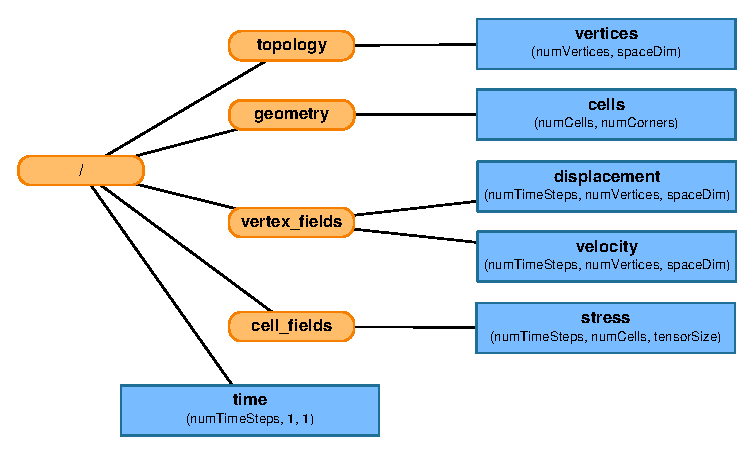
\includegraphics{runpylith/figs/hdf5layout}
\par\end{centering}

\caption{General layout of a PyLith HDF5 file. The orange rectangles with rounded
corners identify the groups and the blue rectangles with sharp corners
identify the datasets. The dimensions of the data sets are shown in
parentheses. Most HDF5 files will contain either \texttt{vertex\_fields}
or \texttt{cell\_fields} but not both. \label{fig:hdf5:layout}}
\end{figure}

\par\end{center}

See Table \vref{tab:material-model-statevars} in Section \vref{sec:material:parameters}
for a table of component values for tensor output in HDF5 files. To
avoid confusion about the ordering of components for tensor data,
we separate the components in the Xdmf file.

HDF5 files do not contain self-correcting features that allow a file
to be read if part of a dataset is corrupted. This type of error can
occur if a job terminates abnormally in the middle or at the end of
a simulation on a large cluster or other parallel machine. Fortunately,
HDF5 also offers the ability to store datasets in external binary
files with the locations specified by links in the HDF5 file. Note
that the use of external data files results in one data file per dataset
in addition to the HDF5 and Xdmf files. The external data files use
the name of the HDF5 file with the dataset name added to the prefix
and the \texttt{.h5} suffix replaced by \texttt{.dat}. The HDF5 files
include relative paths to the external data files, so these files
can also be moved, but they, too, must be kept together in the same
directory. This provides a more robust method of output because one
can generate an HDF5 file associated with the uncorrupted portions
of the external data files should an error occur. Currently, PyLith
does not include a utility to do this, but we plan to add one in a
future release. Thus, there are two options when writing PyLith output
to HDF5 files: (1) including the datasets directly in the HDF5 files
themselves or (2) storing the datasets in external binary files with
just metadata in the HDF5 files. Both methods provide similar performance
because they will use MPI I/O if it is available. 
\begin{quote}
\textbf{\textcolor{red}{Warning:}}\textbf{ }Storing the datasets within
the HDF5 file in a parallel simulation requires that the HDF5 library
be configured with the \texttt{-{}-enable-parallel} option. The binary
PyLith packages include this feature and it is a default setting in
building HDF5 via the PyLith Installer.
\end{quote}
Accessing the datasets for additional analysis or visualization is
nearly identical in the two methods because the use of external data
files is completely transparent to the user except for the presence
of the additional files. Note that in order for ParaView to find the
HDF5 and external data files, it must be run from the same relative
location where the simulation was run. For example, if the simulation
was run from a directory called ``work'' and the HDF5/Xdmf files
were written to ``work/output'', then ParaView should be run from
the ``work'' directory. See Table \vref{tab:material-model-statevars}
in Section \vref{sec:material:parameters} for a table of component
values for tensor output.


\subsubsection{HDF5 Utilities}

HDF5 includes several utilities for examining the contents of HDF5
files. \texttt{h5dump} is very handy for displaying the hierarchy,
dimensions of datasets, attributes, and even the dataset values. 
\begin{quote}
Dump the entire HDF5 file to stdout (not practical or useful for large
files):
\begin{lyxcode}
h5dump mydata.h5
\end{lyxcode}
Dump the hierarchy of an HDF5 file to stdout:
\begin{lyxcode}
h5dump -n mydata.h5
\end{lyxcode}
Dump the hierarchy with dataset dimensions and attributes to stdout:
\begin{lyxcode}
h5dump -H mydata.h5
\end{lyxcode}
Dump dataset 'vertices' in group '/geometry' to stdout:
\begin{lyxcode}
h5dump -d /geometry/vertices mydata.h5
\end{lyxcode}
\end{quote}
We have also include a utility \texttt{pylith\_genxdmf} (see Section
\vref{sub:pylith_genxdmf}) that generates an appropriate Xdmf file
from a PyLith HDF5 file. This is very useful if you add fields to
HDF5 files in post-processing and wish to view the results in ParaView
or Visit.


\subsubsection{DataWriterHDF5 Parameters}

This HDF5 writer stores the datasets inside the HDF5 file and the
parameters are:
\begin{description}
\item [{filename}] Name of HDF5 file (the Xdmf filename is generated from
the same prefix).
\end{description}

\subsubsection{DataWriterHDF5Ext Parameters}

This HDF5 writer stores the datasets using external data files (a
more robust method for parallel runs) and the parameters are:
\begin{description}
\item [{filename}] Name of HDF5 file (the external dataset filenames and
the Xdmf filename are generated from the same prefix).
\end{description}
An example of changing the writer from the default VTK writer to the
HDF5 writer with external datasets for output over the domain in a
\texttt{.cfg} file is
\begin{lyxcode}
{[}pylithapp.timedependent.domain.output{]}

output\_freq = time\_step

time\_step = 1.0{*}yr

cell\_data\_fields = {[}displacement,velocity{]}

writer = pylith.meshio.DataWriterHDF5Ext

writer.filename = dislocation.h5
\end{lyxcode}

\section{Tips and Hints\label{sec:Tips:Hints}}


\subsection{Tips and Hints For Running PyLith}
\begin{itemize}
\item Examine the examples for a problem similar to the one you want to
run and dissect it in detail.
\item Start with a uniform-resolution coarse mesh to debug the problem setup.
Increase the resolution as necessary to resolve the solution fields
of interest (resolving stresses/strains may require a higher resolution
than that for resolving displacements).
\item Merge materials using the same material model. This will result in
only one VTK or HDF5 file for each material model rather than several
files.
\item The rate of convergence in quasi-static (implicit) problems can sometimes
be improved by renumbering the vertices in the finite-element mesh
to reduce the bandwidth of the sparse matrix. PyLith can use the reverse
Cuthill-McKee algorithm to reorder the vertices and cells.
\item If you encounter errors or warnings, run \texttt{pylithinfo} or use
the \texttt{-{}-help}, \texttt{-{}-help-components}, and \texttt{-{}-help-properties}
command-line arguments when running PyLith to check the parameters
to make sure PyLith is using the parameters you intended.
\item Use the \texttt{-{}-petsc.log\_}view, \texttt{-{}-petsc.ksp\_monitor},
\texttt{-{}-petsc.ksp\_view}, \texttt{} \\
\texttt{-{}-petsc.ksp\_converged\_reason}, and \texttt{-{}-petsc.snes\_converged\_reason}
command-line arguments (or set them in a parameter file) to view PyLith
performance and monitor the convergence.
\item Turn on the journals (see the examples) to monitor the progress of
the code.
\end{itemize}

\subsection{Troubleshooting\label{sec:Troubleshooting}}
\begin{itemize}
\item Consult the PyLith FAQ webpage (\url{http://www.geodynamics.org/cig/community/workinggroups/short/workarea/pylith-wiki})
which contains a growing list of common problems and their corresponding
solutions.
\item \texttt{ImportError: liblapack.so.2: cannot open shared object file: No
such file or directory}\end{itemize}
\begin{quote}
PyLith cannot find one of the libraries. You need to set up your environment
variables (e.g., PATH, PYTHONPATH, and LD\_LIBRARY\_PATH) to match
your installation. If you are using the PyLith binary on Linux or
Mac OS X, run the command \texttt{source setup.sh }in the directory
where you unpacked the distribution. This will set up your environment
variables for you. If you are building PyLith from source, please
consult the instructions for building from source.\end{quote}
\begin{itemize}
\begin{singlespace}
\item \texttt{>\textcompwordmark{}> \{command line\}:: } \\
\texttt{-{}- pyre.inventory(error) } \\
\texttt{-{}- p4wd <- 'true' } \\
\texttt{-{}- unrecognized property 'p4wd' } \\
\texttt{>\textcompwordmark{}> \{command line\}:: } \\
\texttt{-{}- pyre.inventory(error) } \\
\texttt{-{}- p4pg <- 'true' } \\
\texttt{-{}- unrecognized property ' p4pg'}\end{singlespace}
\end{itemize}
\begin{quote}
Verify that the `mpirun' command included in the PyLith package is
the first one on your PATH:

\texttt{\$ which mpirun}

If it is not, adjust your PATH environment variable accordingly.\end{quote}
\begin{itemize}
\item \texttt{\textquotedbl{}merlin.DistributionNotFound: Cheetah\textquotedbl{}
error}\end{itemize}
\begin{quote}
This error occurs when trying to use the 32-bit linux binary on some
64-bit linux systems. One of the Python packages PyLith uses does
not know how to determine the system architecture at runtime. The
workaround is:
\begin{enumerate}
\item Go to the \texttt{lib/python2.7/site-packages} directory.
\item Unzip \texttt{merlin-1.8-py2.7.egg} (if it is a file and not a directory).
\item Go to the merlin directory.
\item Edit \texttt{\_\_init\_\_.py}. Replace line 308 plat = get\_platform()
with plat = \textquotedbl{}linux-i686\textquotedbl{}
\item If \texttt{merlin-1.8-py2.7.egg} is a file, rezip merlin. Go to the
site-packages directory and enter \textquotedbl{}\texttt{zip -r merlin-1.8-py2.7.egg
merlin}\textquotedbl{}.
\end{enumerate}
\end{quote}
\begin{itemize}
\item \texttt{-{}- Solving equations.} \\
\texttt{{[}0{]}PETSC ERROR: -{}-{}-{}-{}-{}-{}-{}-{}-{}-{}-{}-{}-{}-{}-{}-
Error Message -{}-{}-{}-{}-{}-{}-{}-{}-{}-{}-{}-{}-{}-{}-{}-{}-{}-{}-{}-{}-{}-{}-{}-{}-{}-{}-{}-{}-{}-{}-
} \\
\texttt{{[}0{]}PETSC ERROR: Detected zero pivot in LU factorization} \\
\texttt{ see http://www.mcs.anl.gov/petsc/petsc-as/documentation/faq.html\#ZeroPivot!}\end{itemize}
\begin{quote}
This usually occurs when the null space of the system Jacobian is
nonzero, such as the case of a problem without Dirichlet boundary
conditions on any boundary. If this arises when using the split fields
and algebraic multigrid preconditioning, and no additional Dirichlet
boundary conditions are desired, then the workaround is to revert
to using the Additive Schwarz preconditioning without split fields
as discussed in Section \vref{sec:petsc:options}. \end{quote}
\begin{itemize}
\item PyLith crashes with a bus error.\end{itemize}
\begin{quote}
This often indicates that PyLith is using incompatible versions of
libraries. This can result from changing your environment variables
after configuring or installing PyLith (when building from source)
or from errors in setting the environment variables (PATH, LD\_LIBRARY\_PATH,
and PYTHONPATH). If the former case, simply reconfigure and rebuild
PyLith. In the latter case, check your environment variables (order
matters!) to make sure PyLith finds the desired directories before
system directories. \end{quote}
\begin{itemize}
\item PyLith crashes with a segmentation fault.\end{itemize}
\begin{quote}
A segmentation fault might be caused by an error that wasn't trapped
or a bug in the code. Please report these cases so that we can fix
these problems (either trap the error and provide the user with an
informative error message, or fix the bug). If this occurs with any
of the problems distributed with PyLith, simply submit a bug report
(see Section \vref{sec:Getting-Help-and}) indicating which problem
you ran and your platform. If the crash occurs for a problem you created,
it is a great help if you can try to reproduce the crash with a very
simple problem (e.g., adjust the boundary conditions or other parameters
of one of the examples to reproduce the segmentation fault). Submit
a bug report along with log files showing the backtrace from a debugger
(e.g., gdb) and the valgrind log file (only available on Linux platforms).
You can generate a backtrace using the debugger by using the \texttt{-{}-petsc.start\_in\_debugger}
command-line argument:\end{quote}
\begin{lyxcode}
pylith {[}..args..{]} -{}-petsc.start\_in\_debugger

(gdb) continue

(gdb) backtrace\end{lyxcode}
\begin{quote}
To use valgrind to detect the memory error, first go to your working
directory and run the problem with \texttt{-{}-launcher.dry}:\end{quote}
\begin{lyxcode}
pylith {[}..args..{]} -{}-launcher.dry\end{lyxcode}
\begin{quote}
Instead of actually running the problem, this causes PyLith to dump
the mpirun/mpiexec command it will execute. Copy and paste this command
into your shell so you can run it directly. Insert the full path to
valgrind before the full path to mpinemesis and tell valgrind to use
a log file:\end{quote}
\begin{lyxcode}
{\footnotesize{}mpirun -np 1 /path/to/valgrind -{}-log-file=valgrind-log  /path/to/mpinemesis -{}-pyre-start {[}..lots of junk..{]}}{\footnotesize \par}
\end{lyxcode}

\section{Post-Processing Utilities}

The PyLith distribution includes a few post-processing utilities.
These are Python scripts that are installed into the same bin directory
as the \texttt{pylith} executable.


\subsection{\texttt{pylith\_eqinfo}}

This utility computes the moment magnitude, seismic moment, seismic
potency, and average slip at user-specified time snapshots from PyLith
fault HDF5 output. The utility works with output from simulations
with either prescribed slip and/or spontaneous rupture. Currently,
we compute the shear modulus from a user-specified spatial database
at the centroid of the fault cells. In the future we plan to account
for lateral variations in shear modulus across the fault when calculating
the seismic moment. The Python script is a Pyre application, so its
parameters can be specified using \texttt{.cfg} and command line arguments
just like PyLith. The Pyre properties and facilities include:
\begin{description}
\item [{output\_filename}] Filename for output of slip information.
\item [{faults}] Array of fault names.
\item [{filename\_pattern}] Filename pattern in C/Python format for creating
filename for each fault. Default is\\
\texttt{output/fault\_\%s.h5}.
\item [{snapshots}] Array of timestamps for slip snapshosts ({[}-1{]} means
use last time step in file, which is the default).
\item [{snapshot\_units}] Units for timestamps in array of snapshots.
\item [{db\_properties}] Spatial database for elastic properties.
\item [{coordsys}] Coordinate system associated with mesh in simulation.
\end{description}

\subsection{\texttt{\label{sub:pylith_genxdmf}pylith\_genxdmf}}

This utility generates Xdmf files from HDF5 files that conform to
the layout used by PyLith. It is a simple Python script with a single
command line argument, the HDF5 file for input. Typically, it is sued
to regenerate Xdmf files that get corrupted or lost due to renaming
and moving. It is also useful in updating Xdmf files when users add
fields to HDF5 files during post-processing.
\begin{lyxcode}
pylith\_genxdmf -{}-file=\textit{PYLITH\_HDF5\_FILE}\end{lyxcode}
\begin{quote}
\textbf{\textcolor{red}{Warning:}}\textbf{ }If the HDF5 files contain
external datasets, then this utility should be run from the same relative
path to the HDF5 files as when they were created. For example, if
a PyLith simulation was run from directory \texttt{work} and HDF5
files were generated in \texttt{output/work}, then the utility should
be run from the directory \texttt{work}. Furthermore, a visualization
tool, such as ParaView, should also be started from the working directory
\texttt{work}.\end{quote}

